\chapter{Learning to learn}
\begin{quotation}
\noindent ``\emph{quote}''
\begin{flushright}\textbf{author}\end{flushright}
\end{quotation}

\vspace*{0.5cm}

Developing and tuning algorithms to find the optimal strategy to solve a
reinforcement learning problem is hard. Some of the challenges one meets are:
\begin{itemize}
	\item the tradeoff between exploration and exploitation
	\item designing a strategy that allows for versatile training
	\item choosing hyperparameters \todo{define} that make the strategy
		optimal considering the reinforcement learning problem at hand
\end{itemize}

Let us consider the problem of learning a simple bandit problem with dependent
arms. Say, for example, that a bandit has two arms, each of which producing
a reward according to a Bernoulli distribution with the following parameters :
$$ \begin{cases} P(r \mid \text{arm}_1) = p_b \\ 
P(r \mid \text{arm}_2) = 1 - p_b  \end{cases} $$
where $P(r \mid \text{arm}_1)$ is the probability of arm 1 to generate a reward
and $0 \leq p_b \leq 1$ is the parameter of the bandit problem. One way to
solve this problem would be to use the $\epsilon$-greedy strategy. This
strategy keeps an average of the reward of each earm and chooses the next
action the following way : choose the action with the best average
reward so far with probability $(1-\epsilon)$, otherwise choose a random action.
This raises the question about choosing $\epsilon$. Choosing a low $\epsilon$
encourages exploitation but we have a higher chance of wrongly estimating $p_b$.
Choosing a high $\epsilon$ doesn't allow the agent to perform optimally once
its knowledge about the parameters of the problem is likely to be optimal.
Moreover, we could choose a variable $\epsilon$, high at first but slowly
converging to 0, but we then are faced with the choice of another
hyperparameter : the number of steps over which $\epsilon$ should be annealed.\\

One could propose using a more advanced method, and there are many. Multi-armed
bandits have been heavily studied and to this day, several algorithms exist to
solve the kind of bandit problems defined above very quickly - i.e. to explore
just enough to implicitly learn $p_b$ so to exploit the best arm as much as
possible. Examples of these algorithms are the Gittins indices algorithm
\cite{Gittins79banditprocesses},
UCB \cite{Auer:2002:FAM:599614.599677} and Thompson sampling
\cite{thompson1933}.\\

The obvious problem here is that we can always choose to manually design more
and more sophisticated techniques and to tune more perfectly their parameters,
but could we not instead use reinforcement learning to do this for us instead?\\

Recently, Wang et al. \cite{learningtorl} and Duan et al. \cite{fastrlviaslowrl}
proposed the idea of using reinforcement learning to learn an algorithm which
deploys an optimal strategy for a class of problems sharing a similar structure.
We will use the name "meta-RL" or meta-learning for this technique, as proposed 
by Wang et al.\\

\begin{figure}
	\centering
	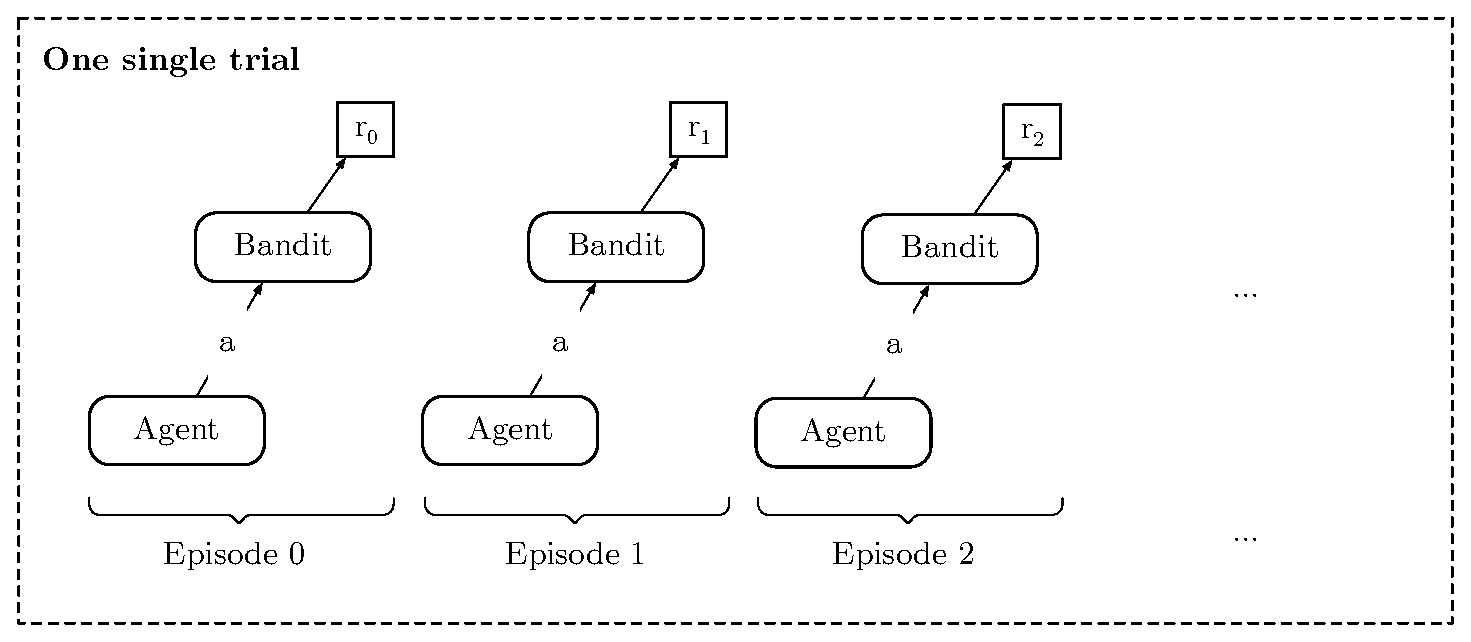
\includegraphics[width=0.7\linewidth]{fig/normal_bandit_training.eps}
	\caption{A classic training sequence to learn a bandit problem}
	\label{fig:normal_bandit_training}
\end{figure}

In classic reinforcement learning (see Figure~\ref{fig:normal_bandit_training}),
the goal of the agent is to maximise its
expected reward for each episode; for this, we let the agent play several
episodes, choosing actions according to a policy which is learned over time, 
but of which the learning process is manually defined by a strategy (Gittins,
UCB, ...) hoping that the agent will yield high rewards as fast as possible.
The part of this process we are interested in is the hand-designed updating of
the policy inbetween episodes.\\

As stated at the beginning of this chapter, designing strategies to learn
policies is a hard task and can demand a sensitive tuning of parameters.
Instead of manually designing ways to make the agent succeed faster, in meta-RL,
the agent plays a trial of several episodes of the same problem and has to
maximise its expected reward across all episodes of a trial (see 
Figure~\ref{fig:meta_bandit_training}). This will incentivize the agent
to understand the structure of a problem and develop a strategy that allows it 
to estimate the parameters of the problem as fast as possible.\\

\begin{figure}
	\centering
	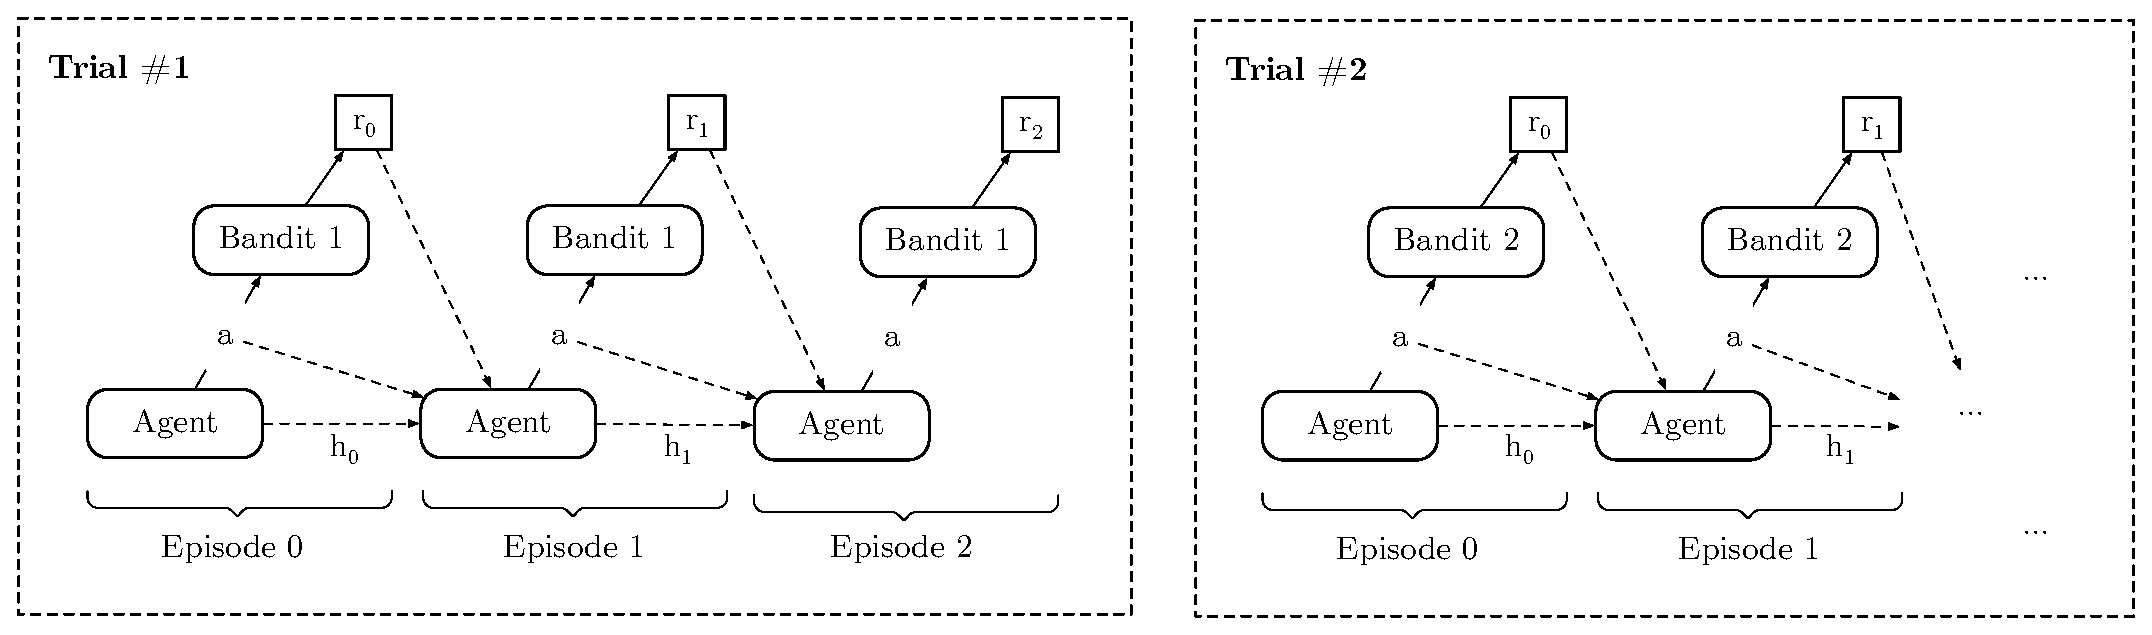
\includegraphics[width=\linewidth]{fig/meta_bandit_training.eps}
	\caption{The training sequence for a meta-RL agent on a bandit problem}
	\label{fig:meta_bandit_training}
\end{figure}

In our manually designed strategies, we use previous actions and rewards
to update the policy and make it better. Similarly, in order to
make meta-RL work, the agent has to receive as input the previous reward
and the action that led to that reward, but it also needs to carry on some
sort of memory of past actions and rewards.\\


\begin{figure}
	\centering
	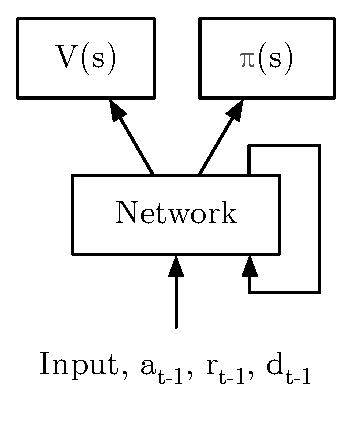
\includegraphics[width=0.2\linewidth]{fig/a2c_meta.eps}
	\caption{The meta-learning A2C agent}
	\label{fig:a2c_meta}
\end{figure}

\begin{figure}
	\centering
	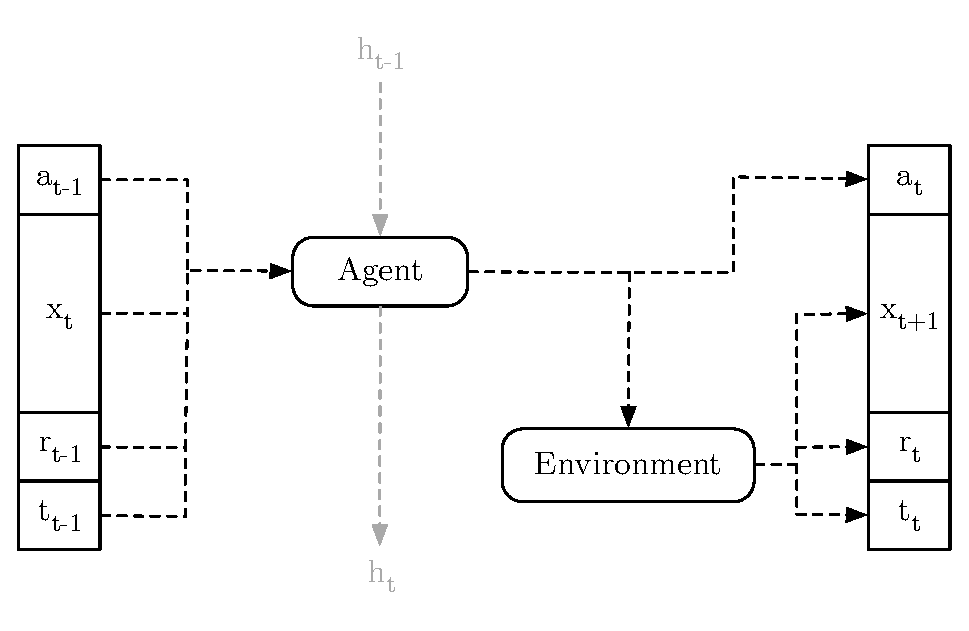
\includegraphics[width=0.6\linewidth]{fig/meta_rl_timestep.eps}
	\caption{An unrolled timestep in the meta-RL training setting. At each
	timestep, the agent receives an observation of the state of the
	environment as well as the previous action taken, the associated reward,
	and the termination flag. It also receives its previous hidden state
	if and only if the previous timestep was part of the same trial (this
	could still mean that the last timestep was from a different episode
	which just terminated)}
	\label{fig:meta_rl_timestep}
\end{figure}

The general setup presented by Wang et al. uses a recurrent neural network of
which the weights, once trained "slowly" over several trials of multiple
episodes, will encode the "fast" training policy.
Figure \ref{fig:a2c_meta} shows the meta-learning A2C agent presented in Wang
et al. \cite{learningtorl}. There are two differences to note compared to
Figure~\ref{fig:a2c}: the first one is the recurrent connection, and the
second one is the set of values we input to the agent at each time step. In
addition to the state of the environment, we add the previous action, 
previous reward and a termination flag which is set to 1 when an episode
has reached a terminal state; 0 otherwise.\\

It is important to emphasize on the fact that the agent passes on its hidden
state between different episodes of the same trial (and if episodes last for
more than one timestep, between timesteps as well), but \textbf{not} between
trials (see Figure~\ref{fig:meta_bandit_training}).
The reason why the inter-episode connection is needed is because
the agent might want to deploy a different policy given the results of 
previous episodes as it has to optimise its expected reward across multiple
episodes.

\todo{Talk about bandit results?}

\section{Meta-learning CartPole}
\label{section:setting}
We will study the performance of meta-learning on various distributions of 
the CartPole problem. The CartPole environment describes a cart, rolling on 
a frictionless rail. A pole is attached to the cart and has to be kept balanced
above the cart for more than 195 timesteps by also keeping the cart within a 
defined section of the rail. The agent has two actions at its disposal: nudge
the cart left or right. The observation of the state is a 4-valued vector 
containing the position of the cart, its velocity, the angle of the pole and
the velocity of the pole at its tip. At each time step, the environment emits
a reward of +1; so if the agent keeps the pole and the cart in their 
respective acceptable ranges for 20 timesteps, it will receive a total reward
of 20.\\
\todo{figure}

\subsection{Generating a distribution of CartPole problems}
To generate a distribution of similar, yet different CartPole problems, we
will play with two different parameters.

\paragraph{Permutations} In standard reinforcement learning, the state
observation vector is always ordered, meaning that each component of the vector
always represents the same value (in CartPole for example, the first component
represents the position of the cart). We can generate a set of $4! = 24$
CartPole problems where for each problem, the state observation vector is
permutated with problem-unique permutation. This means that the agent will
receive a vector of 4 values without knowing which is which.

\paragraph{Actions inversion} We will also introduce the inversion of the
agent's actions. Just like the input vector, the policy output is ordered
(the first component of the policy corresponds to the first action which is
always the same). We will study how inverting actions affects training : instead
of always associating the first component of the policy vector with going left,
we will duplicate each of the 24 problems stated above by inverting the left
and the right action. This adds up to a distribution of 48 CartPole problems.

\begin{figure}
	\centering
	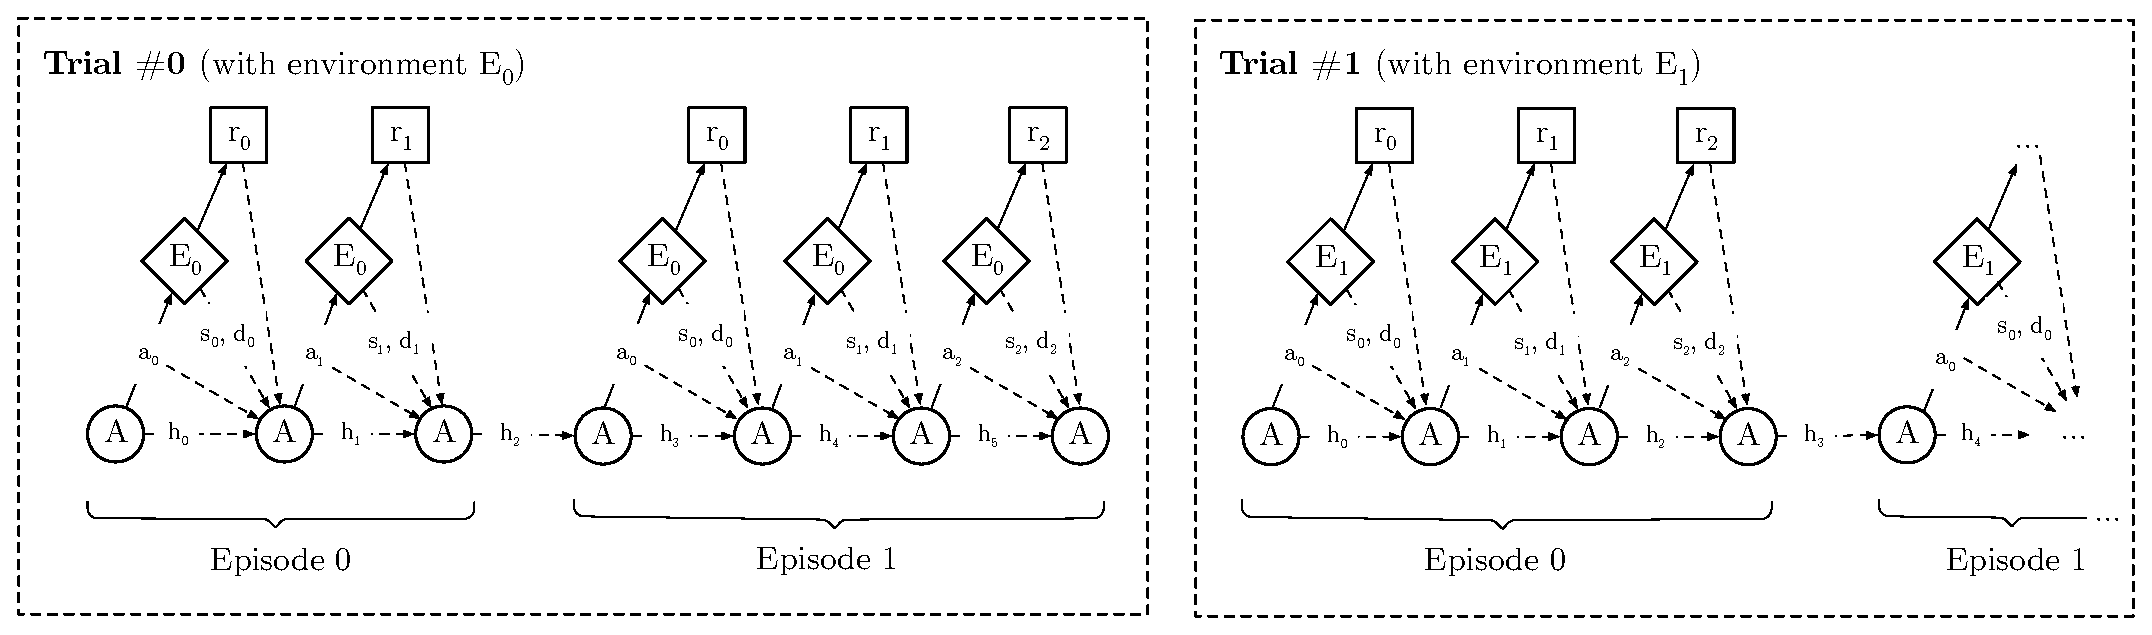
\includegraphics[width=\linewidth]{fig/meta_cartpole.eps}
	\caption{Meta-learning for multi-timestep episodes. A is the agent,
	$E_0$ is the problem selected from the distribution for the duration
	of a trial, $s_t$, $r_t$, $a_t$, $d_t$ and $h_t$  are respectively the state,
	the reward, the action chosen, the termination flag
	and the hidden state at timestep $t$.} 
	\label{fig:meta_cartpole}
\end{figure}

\todo{separate in figure label}

\subsection{Agent architecture}
Our agent is an A2C agent built as described in Figure~\ref{fig:}\todo{fig}.
The input vector is a concatenation of the state observation, the previous
action taken, the reward obtained at the previous timestep and the termination
flag :
$$ i = [s_t, a_{t-1}, r_{t-1}, d_{t-1}] $$
The action taken is converted to a one-hot encoding (converting the action
index into a vector of length $|A|$ containing zeros except a single 1 at the
index of the action). This vector is then fed to a LSTM sized at 48 hidden
units, followed by two branches :
\begin{enumerate}
	\item a fully connected softmax layer with $|A|$ units (the policy
		output)
	\item a fully connected linear layer with 1 unit (the value output).
\end{enumerate}
The loss of the A2C agent is the following : 
$$ \mathcal{L} = \beta_v \mathcal{L}_v + \beta_p \mathcal{L}_p - \beta_e 
 \mathcal{L}_e $$
where $\mathcal{L}_v$ is the value loss : 
$$ \mathcal{L}_v = (R_{t-1} - V(s_t))^2$$
$\mathcal{L}_p$ is the policy loss : 
$$ \mathcal{L}_p = \pi(a_t \mid s_t) (R_t - V(s_t))$$
$\mathcal{L}_e$ is the entropy regularisation : 
$$ \mathcal{L}_e = \sum\limits_{a \in A}\pi(a \mid s_t)\log(\pi(a \mid s_t))$$
and $\beta_v = 0.5$, $\beta_p = 1$, $\beta_e = 0.05$.\\

Unless stated, the discount factor used in all experiments is $\gamma=0.9$. 



